% !TeX root = ../main-paper.tex
\section{Results}

\subsection{Experiment 1: NER sensibility to the number of training samples}

Qualitative results
\textbf{TODO random samples of results + selection of failure cases}


Quantitative results: table + graph ideally (with training set size info)

\begin{table}[!h]
\caption{Models performances vs trainset size}
\centering
\begin{tabular}[t]{lr|cccccccc|}
\toprule
 & Trainset size & 49 & 99 & 199 & 398 & 796 & 1593 & 3186 & 6373\\
 & Trainset size (\%) & 0.8 & 1.5 & 3.1 & 6.2 & 12.5 & 25 & 50 & 100\\
 \hline \hline
\multirow{3}{*}{F1 score} & SpaCy NER & 0.870 & 0.890 & 0.903 & 0.919 & 0.921 & 0.928 & 0.932 & 0.936\\
& CamemBERT & 0.894 & 0.903 & 0.927 & 0.934 & 0.943 & 0.953 & 0.947 & 0.955\\
& CamemBERT+pretraining & 0.900 & 0.914 & 0.929 & 0.934 & 0.942 & 0.945 & 0.948 & 0.954\\
\midrule
\multirow{3}{*}{Precision} & SpaCy NER precision & 0.856 & 0.877 & 0.900 & 0.920 & 0.924 & 0.928 & 0.931 & 0.938\\
& CamemBERT & 0.873 & 0.881 & 0.914 & 0.930 & 0.934 & 0.954 & 0.938 & 0.958\\
& CamemBERT+pretraining & 0.879 & 0.898 & 0.916 & 0.927 & 0.934 & 0.940 & 0.941 & 0.954\\
\midrule
\multirow{3}{*}{Recall} & SpaCy NER & 0.886 & 0.904 & 0.907 & 0.917 & 0.919 & 0.928 & 0.933 & 0.933\\
& CamemBERT & 0.918 & 0.927 & 0.941 & 0.939 & 0.952 & 0.951 & 0.956 & 0.951\\
& CamemBERT+pretraining & 0.922 & 0.930 & 0.943 & 0.942 & 0.950 & 0.951 & 0.955 & 0.954\\
\bottomrule
\end{tabular}
\end{table}

\begin{figure}[htb!]
	   \center{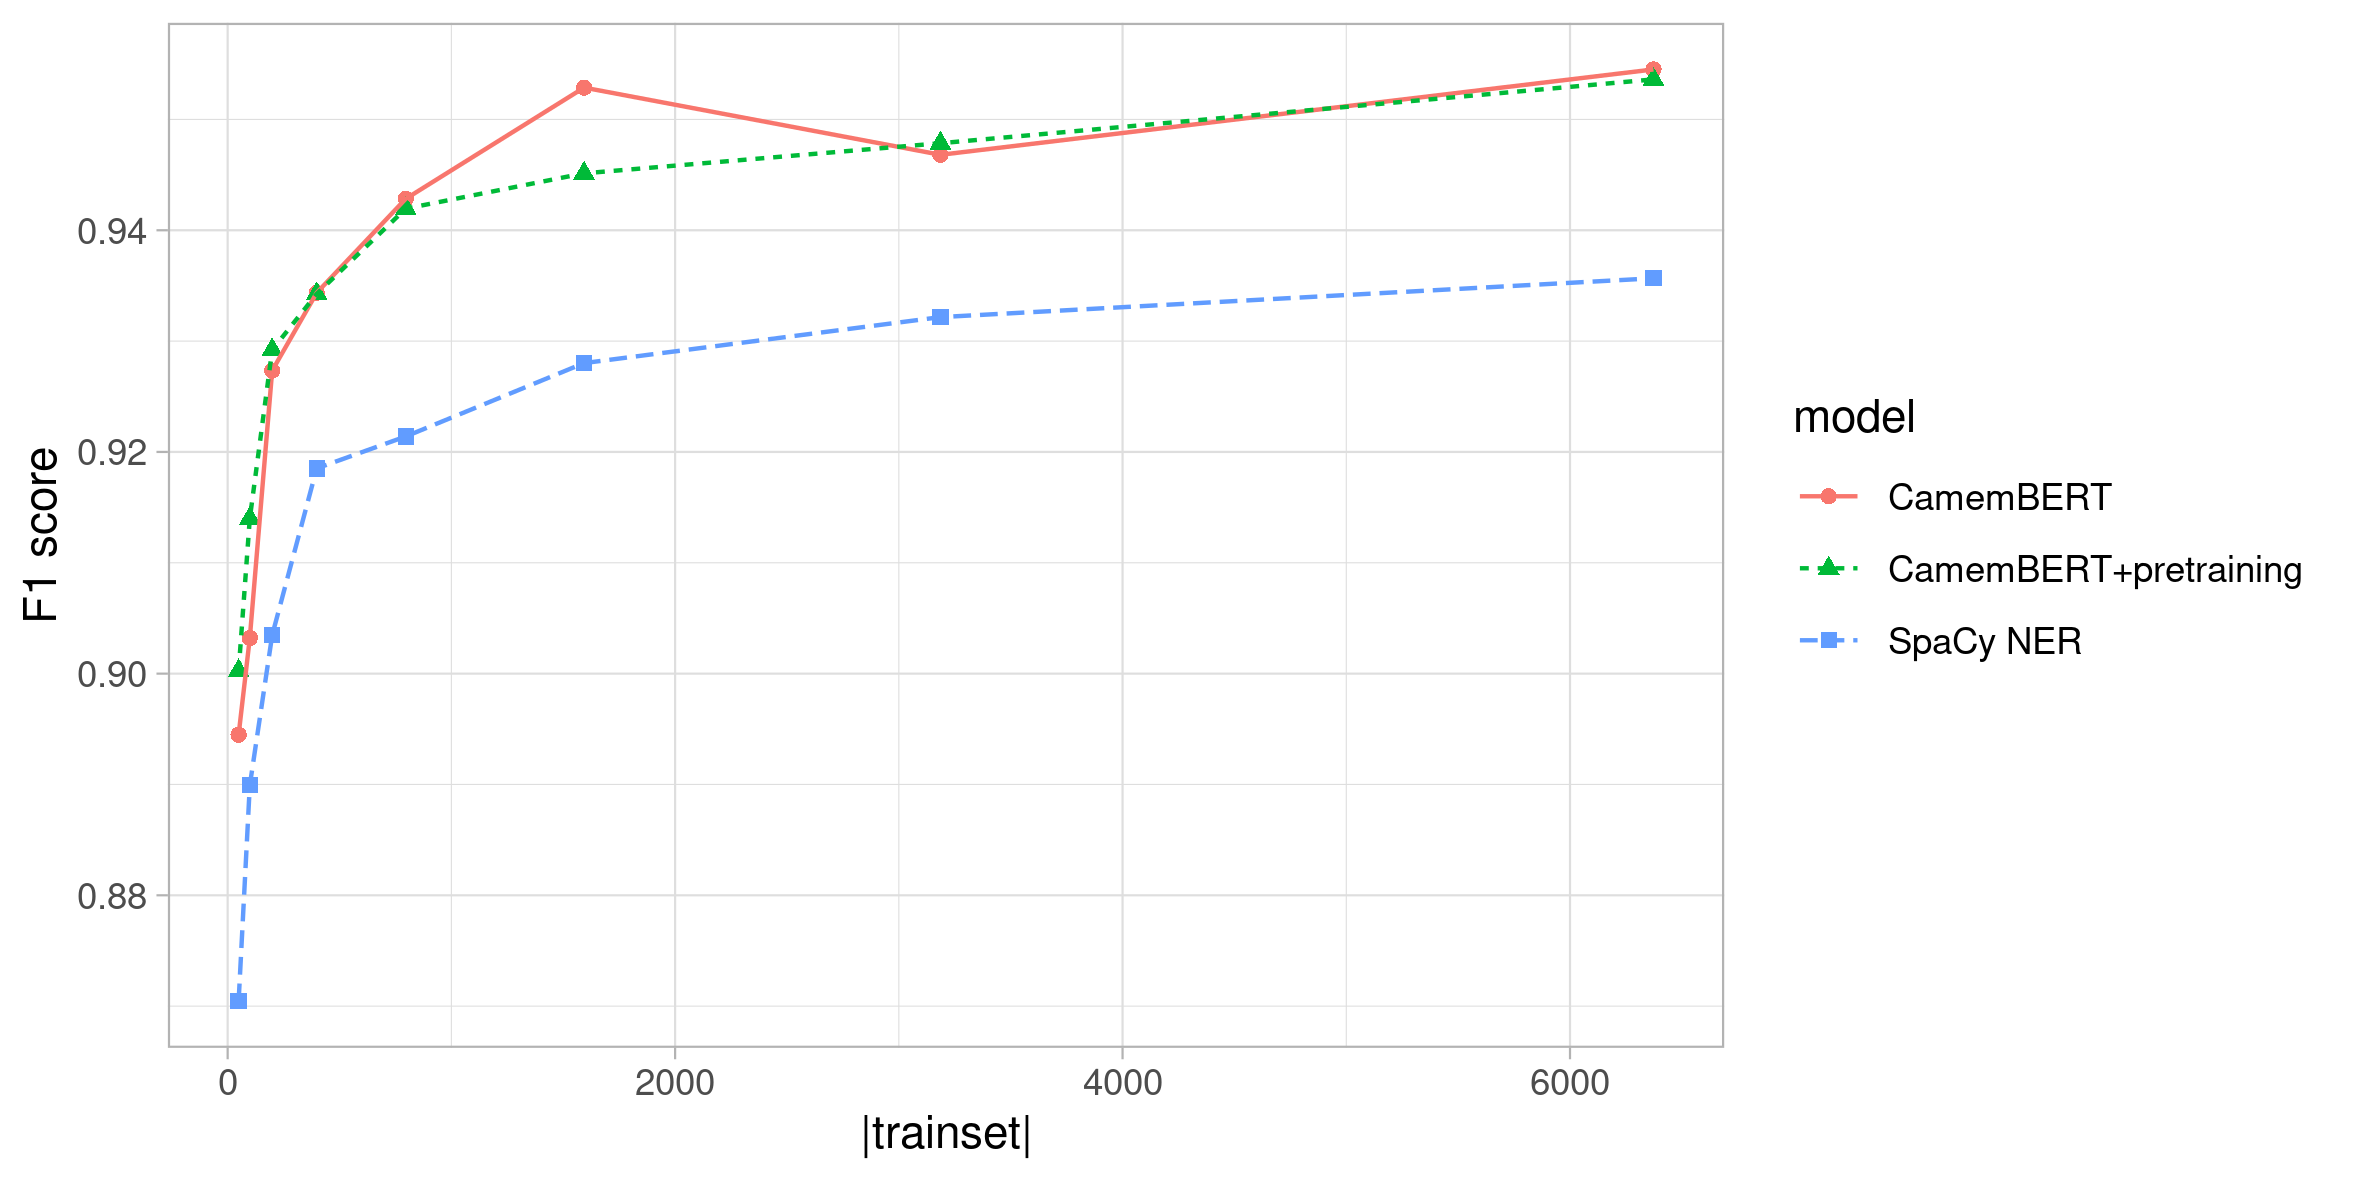
\includegraphics[width=\textwidth]
	       {../material/experiment_1/f1_vs_trainsize.png}}
	  \vspace{3in}
	  \caption{\label{fig:f1-vs-trainsize} Models F1 score on unseen data vs trainset size}
\end{figure}
	                                        


\subsection{Experiment 2: NER in the presence of noisy OCR texts}

Qualitative results
\textbf{TODO random samples of results + selection of failure cases}

Quantitative results: table + graph ideally (with OCR noise, same format as previous)

Table : NER NN models VS train on {noisy, clean} datasets VS evaluate on {noisy, clean} datasets


\begin{table}[h!]
\caption{Camembert vs noise}
\centering
\begin{tabular}{ll|cc|c}
 & & \multicolumn{2}{c|}{Training data} & \\
 & & noisy & clean &   \\ 
\cline{1-4}
\multirow{3}{*}{Test data}& noisy gold (Tesseract) & f1 & f1 & \\
                            & noisy gold (Pero-OCR) & f1 & f1 & \\ 
                            & reference gold & f1 & f1 & \\ 
                            & reference gold & f1 & f1 & \\
\cline{1-4}
\end{tabular}
\end{table}



Opt. use synthetic text perturbation as well? Maybe not interesting and too artificial if we have access to 2+ OCR systems.
(original OCR from BNF, Tesseract 4, Pero OCR…)


\subsection{Discussion}
Interesting points to discuss:
\begin{itemize}
    \item can we train on noisy data? (without manual OCR correction?) => future work? cf Pero OCR training procedure?
    \item do we need better OCR systems or better post-correction techniques (if NER is reliable enough)?
    \item Construction of the lexicon and associated cost
\end{itemize}
